% Chapter 3

\chapter{Expost implementation}  % Main chapter title

\label{Chapter3} % For referencing the chapter elsewhere, use \ref{Chapter2} 

%----------------------------------------------------------------------------------------

% Define some commands to keep the formatting separated from the content 
%\newcommand{\keyword}[1]{\textbf{#1}}
%\newcommand{\tabhead}[1]{\textbf{#1}}
%\newcommand{\code}[1]{\texttt{#1}}
%\newcommand{\file}[1]{\texttt{\bfseries#1}}
%\newcommand{\option}[1]{\texttt{\itshape#1}}


\section{ Introduction}
 We try to characterize truthful implementation in ex post equilibrium in this Chapter.  Due to "Wilson criterion", ex post equilibrium 
 is a good equilibrium in implementation theory for its distribution free property. A large body of literature has been devoted to 
 many aspects of ex post implementation. 

 

 As is pointed out in \parencite{Postlewaite2014}, it is often the case that truthful revelation is not ex post incentive compatible, that is, for a given 
 agent, there are some profiles of the other agents' types for which the agent may be better off by misreporting his type than by 
 truthfully revealing it. However, with the help of money transfer, the authors in \parencite{Maskin00} devised an complicated yet ingenious 
 auction mechanism to Nash implement a rather general kind of allocation problems in interdependent value context. It is obvious 
 that money transfer is one key for implementation. 
 In this chapter, we provide a sufficient and necessary condition for truthful implementation with money transfer. VCG mechanisms in 
 private value context and all its generalized forms in interdependent value context have all successfully find a suitable
 money transfer scheme for specific economic environments. We would like to show the subtlety of those ingenious mechanisms in 
 implementing social goal within our paper's model framework, and how their implemented social goals have satisfied the sufficient and 
 necessary condition.
 Here, for a certain but not rare kind of setting, we propose a simple Generalized Vickery mechanism which can easily make the buyers
 reveal their private information truthfully through the help of money transfer. Of course, the Generalized Vickery mechanism is not 
 balanced scheme. Nevertheless, the ability of the mechanism to make people tell truthfully about their private information is a sign of 
 its power.   
 For the common knowledge part of agents, we make the agents tell truth in Nash equilibrium using insights got from the paper
 \parencite{Repullo90}.
 
 In private value settings, ex post equilibrium is equivalent to dominant strategy
 equilibrium. Thus the well-known VCG mechanism is the ideal mechanism for ex post implementation in private value case. What we care
 most in this paper is the interdependent value setting. We also assume quasilinear utility for the agents, which is a common 
 assumption. 
In \parencite{BergemannM08}, the authors focus on identifying conditions for full implementation
 of a social choice set in ex post equilibrium. They stressed that a conceptual advantage of ex post equilibrium is its 
 robustness to the informational assumptions about the environment. \parencite{Maskin00} proposed an indirect bidding mechanism which
 give ex post partial implementation of the socially efficient outcome.
   An important contribution of \parencite{Maskin00} is that a mechanism for allocating  multiple heterogeneous goods is 
 provided. \parencite{Perry2002} devised another clever mechanism for this case. Their methods consists of a collection of second-price 
 auctions between each pair of bidders conducted over at most two rounds of bidding. Unlike them, in this paper we do not consider 
 full implementation, and for partial implementation we focus on direct revelation mechanism. we use the direct mechanism and get 
 to cover some more situations that are not implementable using the indirect bidding mechanism in \parencite{Maskin00}.
 We restrict out attention to the conditions garanteeing that truthful revelation of one's own private signal constitutes an ex post 
 equilibrium in some carefully designed direct revelation mechanism. That is, we focus on incentive compatibility of truthful
 information revelation in direct mechanism. Partial implementation is enough in this paper. In such direct mechanisms,
 a well devised payment rule is of key importance. \parencite{Ausubel99} provides a payment scheme in its generalized Vickery Auction
 mechanism, which under some conditions achieves the task of implementing social efficiency in ex post equilibrium. 
 \parencite{Jehiel2001} takes into consideration discreet social choice possibilities. 
 
 In this paper, we would like to also investigate the continuous
 cases of interdependent value,  including allocation of continuous resources and efficient provision of continuous public goods. 
 For example, in a room of dancers, a volume must be chosen for the music so that it can provide the best social efficiency. Each person
 has a valuation function of the form 
 $$u_i= v_i(volume) + \alpha_i\sum_{j\neq i}v_j(volume)$$
 Here, the $\alpha_i$ is the altruist coefficient of agent $i$. We will see how to implement social efficiency in this case later in
 the paper. \parencite{Ely2006} is a work dedicated to similar problems. We are going to mention it when we draw on some of their results
 later.


 
 Our intuition is mainly taken from \parencite{Maskin00} Vickery Mechanism and auction theory. 
Simpleness often means less mistakes. Also, a simple mechanism is  easy to supervise. For an outsider, it is not easy to judge who should win the goods in a very complicated mechanism
, so a corrupted social planner might manipulate the result. That is one motivation for us to construct a direct revelation

In interdependent value settings, a winner often suffers from winners' curse. In this paper, we first introduce the notion and model
of interdependent value goods, then for some kind of setting, we find a unique expost Implementation of 
the socially efficient results. Finally, we find an application of the model in the mineral rights assignment problem by aggregating
signals in the designed market.




\section{Key concepts and notations}
First, we give some description of the notations used in this chapter. It's similar to the general framework described in the first chapter. In the meantime of depicting the notations here, we give out the settings for this 
chapter in more detail.
The economic environment consists of
$A$: the set of choice possibilities.

$Z=Z_1\times \dots\times Z_n$:the outcome space. For this chapter, implementation with money transfer means that the 
outcome $z$ has the form $(a, t_1,\cdots,t_n)$ where $a$ is from the set of choice possibilities $A$, $t_i$ is 
the payment agent $i$ has to make.

$U=U_1\times \cdots\times U_n$: the set of all admissible utility functions  $u = \{u_i(\cdot, \cdot)\}_{i=1}^n$ whose 
domain is $Z\times S$. In this paper, quasilinearity is assumed, that is , $u_i((a,t), s)$ takes the form $v_i(a,s)-t_i$. 
$v=\{v_i(\cdot, \cdot)\}_{i=1}^n$ is in a space $V=R^+\times R^+$.

$S=S_1\times \cdots\times S_n$: the set of all admissible signals $s=(s_1,\cdots,s_n)\in S$ that determine types of 
parametric utility functions $u_i(\cdot, s)$, and so it is called the space of signals or called the state of the world. 
In many papers, notation $\theta$ is used in stead of $s$. We adopt the notation $s$ of \parencite{Maskin00} in this paper.
Here, apparently both independent value and interdependent value models are both incorporated in this framework.

$E$: a set of  environments(states of the economy) $e=(\{u_i(\cdot, \cdot)\}_{i=1}^n,s)$. In this paper, 
$e=(\{v_i(\cdot, \cdot)\}_{i=1}^n,s)$ since $v_i$ can identify $u_i$. Moreover,
as will be discussed in the information structure part, the $v$ can be elicit out easily by the social
planner, we simply let $e=s=(s_1,\cdots,s_n)$, which is the decentralized information part of the model that need 
mechanism design to tackle.

The information structure of the paper is specified by

(1)$s_i$is privately observed by agent $i$.

(2)$v=\{v_i(\cdot, \cdot)\}_{i=1}^n$ is common knowledge among the agents.To elicit the common
knowledge part of their information, the social planner can adopt methods similar to those \parencite{Repullo90} propose for Nash
implementation of social choice rules. If very agent reports the same, then the result is believed to be the truth. Otherwise,
some kind of punishment is given to everyone.  

Given economic environments, each agent participates economic activities, makes deci-
sions, receives benefits and pays costs on economic activities.The designer wants to reach
some desired goal that is considered to be socially optimal by some criterion. Let

$F:E\rightarrow \rightarrow Z$: the social goal or called social choice correspondence in which
$F(e)$ is the set of socially desired outcomes at a certain state of the economy under some
criterion of social optimality. For this paper, the social goal is denoted
$$F(s)=\{(a^*,t_1,\cdots,t_n)|a^*\ is\ a \ solution\ to \ \max_a \sum_{i=1}^n v_i(a,s)\}$$
We call this the social goal of efficiency in the paper. Since money transfer is not the concerned part.  we can use 
transfers freely to implement the goal.




 

A mechanism consists of a message space and an outcome function. 

$M_i$: the message space of agent i. 

$M=M_1\times \cdots\times M_n$: the message space in which communications take place.

$m_i \in M_i$: a message reported by agent $i$.

$m=(m_1, \cdots,m_n)\in M$: a profile of Messages.

$h:M\rightarrow Z$: outcome functions that translate messages into an outcome.

$\Gamma=\langle M, h\rangle$: a mechanism.

A very important class of mechanisms is the direct revelation mechanism in which $M_i$ is just the possible world state information 
that agent $i$ has. In this paper, the direct revelation mechanism has a message space $M_i=\{(v, s_i)|v\in V, s \in S \}$. The most
important case of $m$ is where all reported $v$ is the same, and for this case the outcome function can be written as 
$h(m)=(a(v,s),t(v,s))$.

Let $b(e, \Gamma)$ be the set of equilibrium messaging strategies that describes the self-interested behavior of individuals.
For instance, Nash equilibrium $N(e,\Gamma)$ is the most frequently adopted equilibrium concept.

A Mechanism $\langle M, h\rangle$ is said to implement a social choice correspondence $F$ in equilibrium strategy 
$b(e, \Gamma)$ on Environment space $E$ if for every $e\in E$, $h(b(e,\Gamma))\in F(e)$.
Incentive compatibility is another way of saying implementation. A Mechanism is said to be incentive-compatible with a social choice
correspondence $F$ on $E$ if it implements $F$ in some kind of equilibrium on $E$. 








\section{the sufficient and necessary condition for implementation with money transfer}
\begin{prop}


Obviously, for a direct revelation mechanism to implement the social efficiency, every agent must tell truth. 
We give a theorem which is

We assume outside choice is $a_0$, and $v_i(a_0,s)=v_i(a_0,s_{-i})$, that is, the agent $i$'s value of the outside choice does not
depend on $s_i$.
\begin{thm}
The social goal of efficiency can be implemented with money transfers using a generalized VCG 
if and only if 
$$\forall i,\forall s_{-i},\forall a $$
let $\underline{v_i}(a,s_{-i})$ denote
$$ \inf \{v_i(a,s_i, s_{-i})|s_i\ is \ such \ that\ \sum_{j=1}^n v_j(a, s_i, s_{-i}) = \max_{a'} \sum_{j=1}^n v_j(a', s_i, s_{-i}) \}$$
then $v_i(a, s_i,s_{-i})-\underline{v_i}(a,s_{-i})$ is the gain
$$v_i(a(s), s_i,s_{-i})-\underline{v_i}(a,s_{-i})=\max_{s'_i}v_i(a(s'_i,s_{-i})-\underline{v_i}(a(s'_{i},s_{-i}),s_{-i})$$
$$\geqslant \sup \{v_i(a, s_i, s_{-i})|s_i\ is \ such \ that\ \sum_{j=1}^n v_j(a, s_i, s_{-i}) < \max_{a'} \sum_{j=1}^n v_j(a', s_i, s_{-i}) \}$$
Assume that the maximization on $A$ exists,for example, when $A$ is finite. 
\end{thm}
\begin{proof}
Sufficiency:

We need to construct the generalized Vickery Mechanism and then show that it indeed implements the social efficiency.

Step 1. Every agent reports a $(v,s_i)$ from the set $V\times S_i$;

Step 2. If $v$ reported by $n-1$ agent is the same, then go to step 3; otherwise the result is that an  $a_0\in A$ is chosen as exogenous

choice and the process ends.

Step 3. Let $v$ be the same report by $n-1$ agents, then solve the maximization problem

$$\max_{a'} \sum_{j=1}^n v_j(a', s_i, s_{-i})$$


let $a*$,  the solution, be the social planner's choice(If there are more than one solution, randomize among them with equal probability).
let
$$\underline{v_i}=$$
$$ \inf \{v_i(a*,s_i, s_{-i})|s_i\ is \ such \ that\ \sum_{j=1}^n v_j(a*, s_i, s_{-i}) = \max_{a'} \sum_{j=1}^n v_j(a', s_i, s_{-i}) \}$$

The payment each agent i has to make is decided by
$$\underline{v_i}-v_i(a_0,s)$$

Necessity:
We will show the necessity of the condition by way of contradiction. 

Suppose the condition is not met, then we will show that no payment scheme can ensure truthful report in a Nash equilibrium.

First, see that if 
$$t_i> \underline{v_i}-v_i(a_0,s_{-i})$$
Then to get the outside choice, the agent i would rather withdraw in the second step than reporting the truth in the third step  
for certain $s_i$ where $v_i(a*, s)-v_i(a_0,s_{-i}) <t_i$. Such $s_i$ is ensured to exist 
since $t_i> \underline{v_i}-v_i(a_0,s_{-i})$.

Second,denote
$$\sup \{v_i(a, s_i, s_{-i})|s_i\ is \ such \ that\ \sum_{j=1}^n v_j(a, s_i, s_{-i}) < \max_{a'} \sum_{j=1}^n v_j(a', s_i, s_{-i})\}$$
as$\overline{v_i}$
see that if 

$$t_i<\overline{v_i}-v_i(a_0,s_{-i})$$ 

then for some $s_i$

\end{proof}

In order to facilitate the proof, we give the following fundamental theorem of this paper.
It is roughly saying that the value sum of you pretending another type(who have different value when truth telling)
and that type pretending you is less than the value sum of 
you and that type truthfully report your types.
\begin{lemma}[single crossing condition]\label{thm}
A social goal of efficiency $G$ can be implememted on $E$  by some mechanism if and only if $\forall s, \forall v, \forall i$, when 
$v_i(a(v,s), s)\neq v_i(a(v,s'),s')$ where  $s=(s_i, s_{-i})$ and 
$s'=(s'_i, s_{-i})$ (i.e., they only differ in agent's private signal), then

\begin{equation*}\label{equ}
v_i(a(v,s'),s)-v_i(a(v,s), s)<v_i(a(v,s'),s')-v_i(a(v,s), s')
\end{equation*}

\end{lemma}
\begin{proof}
sufficiency: we only need to construct a direct revelation mechanism to implement the social goal of 
efficiency. What we need to do is to construct the money transfer amount. We start from agent 1, $\forall s_{-i}^*$, partition
$s_i$ according to $v_i(a(v,s_i,s_{-i}^*),s_i,s_{-i}^*)$, then as a start point, set 
$t(a(v,s_i,s_{-i}^*),s_i,s_{-i}^*)=t^*\quad\forall s_i $  where $s_i$ is in the partition of $s_i^*$. For those partition of 
signals $s'_i$ that has a higher $v_i(a(v,s'_i,s_{-i}^*),s'_i,s_{-i}^*)$, set $t(a(v,s'_i,s_{-i}^*),s'_i,s_{-i}^*)=t^*+\delta(s_i)$
such that $v_i(a(v,s'),s)-v_i(a(v,s), s)<\delta(s_i)<v_i(a(v,s'),s')-v_i(a(v,s), s')$

set 

$$t_i(v,s)<t_i(v,s')$$
\begin{eqnarray*}
&& v_i(a(v,s'),s)-v_i(a(v,s), s)<t_i(v,s')-t_i(v,s)<v_i(a(v,s'),s')-v_i(a(v,s), s') \\
 && \Longleftrightarrow \\
&& v_i(a(v,s'),s)-t_i(v,s')<v_i(a(v,s), s)-t_i(v,s) \\
&& \quad and\quad v_i(a(v,s), s')-t_i(v,s)<v_i(a(v,s'),s')-t_i(v,s')
\end{eqnarray*}
 That means no one will deviate from truth telling at any signal. Thus truthful report is Nash equilibrium.

 Necessity: Because of the revelation principle, we only need to show truthful implementation in a direct revelation
 mechanism implies the condition.
 
 To be finished.
\end{proof}
Before utilizing Lemma 1 to prove Theorem 1, we talk about some intuition 
\begin{proof}[of Theorem 1]
 
\end{proof}

\begin{figure}
  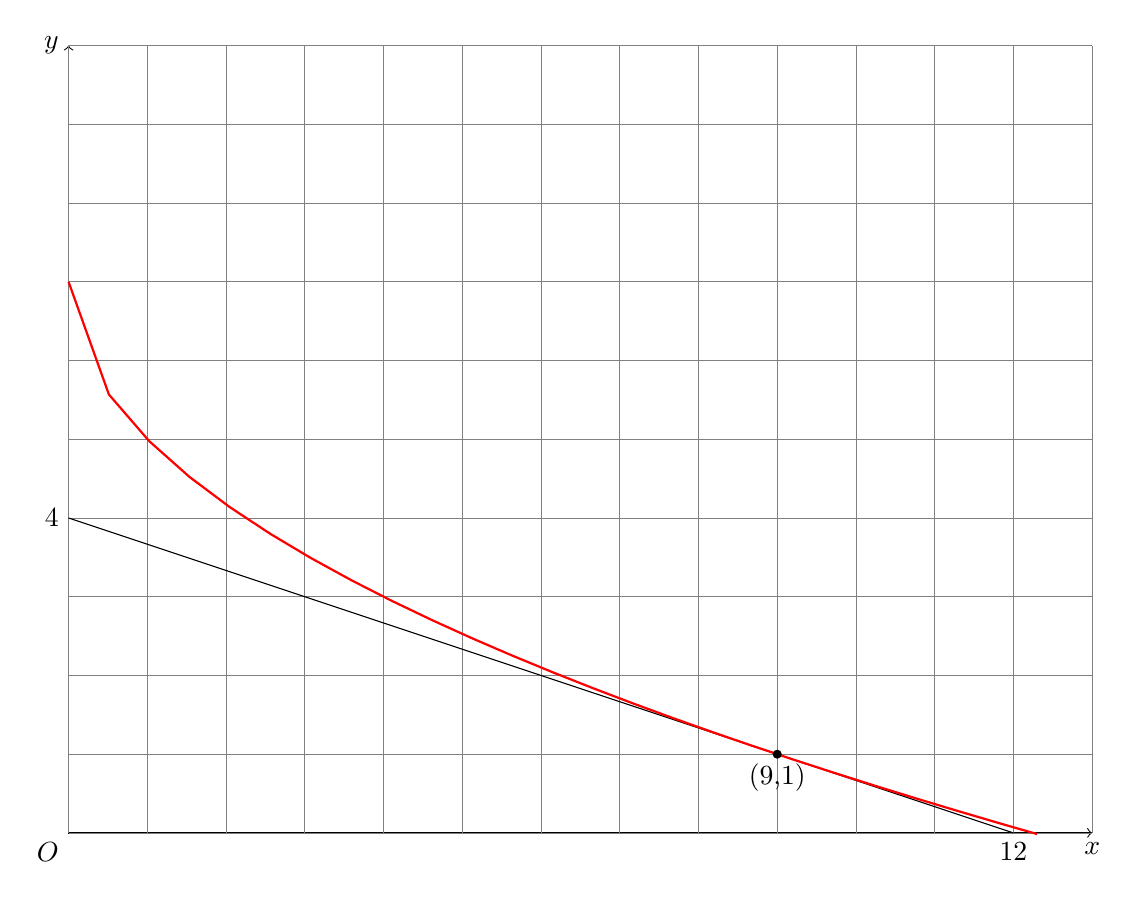
\begin{tikzpicture}
   \draw [<->] (0,10) node [left] {$y$} -- (0,0) node [below left] {$O$} -- (13,0) node [below] {$x$};
   \draw[help lines] (0,0) grid (13,10);

   \draw (0,4) node [left] {4}-- (12,0) node [below] {12};
   \draw [red, thick, domain = 0:12.3] plot (\x,{7-2*sqrt(\x)});
   \draw[fill] (9,1) circle [radius=0.05] node [below] {(9,1)};

  
  \end{tikzpicture}
  \caption{signal payment relation}

 \end{figure}
 Next, we start from a simple task.
\section{continuous cases motivating the establishment of the model}
Let us begin with some examples
\begin{example}
 Consider there are two chess players living $L$ miles apart from each other along a road in a city. They drive their cars to meet
 each other every sunday to play chess face to face, and then go back home. Suppose that they can choose anywhere on the road to meet.
The city governer tries to assign a meeting place minimizing the pollution of their car causing to the city, so he wants to
chose a meeting spot to minimize $c_il_i+c_j(L-l_i)$. They all care about the 
 pollution but they also care about their oil expenditure, player i wants to minimize $v_i= c_il_i+ \alpha(c_il_i+c_j(L-l_i))$. What
 is the transfer scheme that can make the two players telling truth about their private $c_i$ an ex post equilibrium.
\end{example}
when extending the two player game of chess to four player game like bridge, and the four people meet each other,
it is more complicated. 
\begin{example}
 $n$ firms at $n$ corners of a regular n polygon area transporting their produced goods to a city for sale.
The city planner tries to build the city in a place such that it can minimize the pollution caused by transportation of the goods, 
and the firms cares about its own transportation cost as well as the total pollution(the reason why a firm care about pollution
may be that the goods are vegetables and pollution can hurt the production). The oil consumption and thus pollution caused 
by a given amount of goods transportation for each firm is a private value . Each day the goods transported to the city is also
private information for each firm. What is the taxation scheme that can make each firm report their true private information so that the city 
planner can choose the best place to build the city in order to reduce transporation pollution. Here the meaning of the taxation is not
to reduce pollution directly, but to lead the firms to tell truth about their private information such that the planner can choose a
pollution minimizing choice for building the city.
\end{example}

Another economically more interesting example is as following 
\begin{example}
A country has N oligopoly firms producing the same goods ,say oil. They face an exogenous demand function. Competition among them hurt
aggregate profits of the firms. 
The country want to devise a taxation scheme such that every firm reveal their true production cost so that the country can plan
the production quantity for each firms to maximize total profit of the country. This is the private value case that can be implemented
using classical Clark mechanism. 
\end{example}
Now change the scenario to another case where the firms' CEOs know the private cost informations of their own firms. They are all 
shareholders, and all have a large percent of their own firm's stock and a different amount of share on other firms, and these shares
are common knowledge.  Now the valuation of each firm's CEO on the country's production assignment plan are dependent upon all
the cost information and each firm's final production quantity as specified by the country.
 
Now the taxation scheme is a true challenge. In this paper, we try to classify these interdependent value problems into two category,
the ones that can be implemented with money transfer(suitable taxation)in ex post equilibrium, and the ones that can not. For those
that can be implemented with money transfer, we give the taxation scheme that can be used to implement the socially efficient choice.

One interesting finding is that the money transfer scheme is unique up to a shifting constant if the functions involved are
continuously differentiable.

\begin{thm}
Assuming all the partial derivatives exists and are continuous, then solve the following 
differential equations
 $$\frac{\partial t_i}{\partial s_i} = \frac{\partial v_i(a(s_i,s_{-i}),s_i,s_{-i})}{\partial a } \frac{\partial a}{\partial s_i}$$
 $i=1,\cdots,n$ 
 
 gives us a transfer scheme $t(\cdot)$.
A sufficient and necessary condition for implementation with money transfer in such continuous case is that, for all $i$,$s$
by shifting up or down the $t(\cdot,s_{-i})$ to let it be tangent with $ v_i(a(\cdot,s_{-i}),s_i,s_{-i})$ at $s_i$, the curve
$t_i(\cdot,s_{-i})$ is below $ v_i(a(\cdot,s_{-i}),s_i,s_{-i})$, namely, $v_i(a(\cdot,s_{-i}),s_i,s_{-i})-t(\cdot,s_{-i})$ is
maximized at $s_i$.

 
\end{thm}
\begin{proof}
 If truth telling is a ex post equilbrium, it must be the case that $s_i$ is the solution to
 $$\max_{s'_i} \{v_i(a(s'_i,s_{-i}),s_i,s_{-i})-t(s'_i,s_{-i})\}$$
 solving it, we get the conclusions in the theorem.
\end{proof}

The theorem is simple, but it contains much information. One thing is that not every continuously differentiable
social goal $a(s)$ is implementable in ex post equilibrium with money transfer. It must satisfy the conditions in the theorem 
to be implemented with money transfer. The second thing is that even if it can be implemented with money transfer, the scheme for 
implementing it is unique in essence. They only differ by a constant(the solution to the differential equations are some specific
function plus a something of the form $f(s_{-i})$ that is not changing with $s_{-i}$).

Now let us consider the oil producers example. We should give a mathematical structure to it in order to show how the process of mechanism
design is done in this case. Market demand function is $q(p)$, inverse demand function is $p(q)$. The cost function 
facing firm i is $c(q_i,s_i)$, the parameter $s_i$ is privately known. The share of firm $j$
that the leader of firm  $i$ holds is $m_{ij}$, and  the leader $i$ cares the overall profit 
$v_i(q,s)=\sum_{j=1}^{n} m_{ij}(q_jp(q)-c(q_j,s_j))$. The country's goal is 
$$\max_{\{q_1,\cdots,q_n\}}\sum_{j=1}^{n} (q_jp(q)-c(q_j,s_j)) $$
The solution to this maximization problem must satisfy the first order conditions
$$q_j \frac {\partial p(q)}{\partial q}+p(q)=\frac {\partial c(q_j,s_j)}{\partial q_j}$$
$$j=1,\cdots,n$$

For many function forms, the above conditions are also sufficient, and we calculate out ${q_1(s),\cdots,q_n(s)}$ from the above 
equations. Next, by using the conditions in the above theorem, we get 
$$\frac{\partial t}{\partial s_i} = \sum_{j=1}^{n} m_{ij}\{q_j\frac {\partial p(q)}{q}(\frac{\partial q_1}{s_i}+\cdots+\frac{\partial q_n}{s_i})-\frac {\partial c(q_j,s_j)}{\partial q_j}\frac{\partial q_j}{s_i}\}$$
Now that the transfer scheme is calculated, we only need to verify whether it satisfies the requirement that $s_i$ maximizes  
$$\sum_{j=1}^{n} m_{ij}\{q_j(\cdot,s_{-i})p(q(\cdot,s_{-i}))-c(q_j(\cdot,s_{-i}),s_j)\}-t_i(\cdot,s_{-i})$$

For this continuously differentiable situation, the private value case of the problem always has the unique solution, the uniqueness
has been shown by the above more general result. And the unique mechanism is the well-known VCG mechanism. This has been shown by
Laffont and Maskin(Econometrica, 1980). Tian

And for private value case, 
ex post implementation is indeed dominant strategy implementation. A specialness of the private value situation is that the calculated
VCG money transfer mechanism can always satisfy the additional requirement for implementability. We will show why now. 
\section{discrete social goal}
The discrete social choice possibility set $A$ does not allow differential analysis like we do above in the continuous social choice
possibility set case. However, the allocation of discrete social resources, or the determination of whether a project should be carried
are important social choice problem we have to face. We are also interested at whether we can implement such social choices with money
transfer. We start from allocation of one good.

\subsection{allocation of one good }

Imagine the following scenario : there is a group of agents who are familiar with each other, and the social planner has
one good to allocate to one of them. The socially efficient outcome is to give it to the one who 
values it the most. Suppose each agent can only detects one of the qualities of the good, and the total value of the 
good for any agent is only determined by all the qualities of the good and the importance of each quality to the agent 
himself. This is a situation completely covered by our model framework in the previous section. The social choice possibility
set $A=\{(1,0,\cdots,0),\cdots,(0,\cdots,0,1)\}$. Every body only cares about getting the object, and when one does not get it his or
her utility gain is 0 from the allocation. Now what the social planner want is a mechanism to implement the socially efficient outcome. 

\parencite{Maskin00} has partly solved the problem and give us an auction mechanism to implement a rather large economic 
environment set $E$ in this one good allocation environment. However, as the authors pointed out in the footnote 26 of 
their paper, some utility forms can not be implemented by their auction mechanism. In this section, through combining the 
insights of the two authors with the power of revelation mechanism, we try and find a direct revelation mechanism  which
enlarge the $E$ on which the social goal of efficiency $G$ is implementble, for example, the economic environment in footnote
26 of their paper.
In Theorem~\ref{thm}, we have shown what is the sufficient and necessary condition for implementation with money 
transfer. In this simple case, we give some simple assumptions parallel to the sufficient and necessary condition
so that we can implement the social efficiency.

In this one good allocation problem,let $v_i(s)=v_i(\epsilon_i,s)$ where $\epsilon_i$ is the allocation of the good to i. Then we
have the following theorem.
\begin{corollary}[of Theorem 1]
The efficient allocation of one good can be implemented  
if and only if 
 $$\forall i,\forall s_{-i}$$
 $$ \inf \{v_i(s_i, s_{-i})|s_i\ is \ such \ that\ v_i(s_i, s_{-i}) = \max_{j\in\{1,\cdots,n\}}v_j(s_i, s_{-i}) \}$$
 $$\geqslant \sup \{v_i(s_i, s_{-i})|s_i\ is \ such \ that\ v_i(s_i, s_{-i}) < \max_{j\in\{1,\cdots,n\}}v_j(s_i, s_{-i}) \}$$

\end{corollary}
 we try to talk about the meaning the condition.


\begin{assumption}
 $v_i(s)$ is  monotonic with repect to $s_i$, and without loss of generality, we assume it is strictly increasing with $s_i$.
\end{assumption}
This assumption can ensure every different $s_i$ corresponds to a different $v_i(s_i, s_{-i})$. That can simplify analysis. 

\begin{assumption}
When $v_i(s'_i, s_{-i})-v_i(s_i,s_{-i})>0$, then $\forall j\neq i$
$$v_i(s'_i, s_{-i})-v_i(s_i,s_{-i})>v_j(s'_i, s_{-i})-v_j(s_i,s_{-i}) $$
 
\end{assumption}



\begin{prop}
 Under the two Asumptions above, we can implement the social goal of efficiency that the agent who values the good most gets it .
\end{prop}

\begin{proof}
 We only need to find an appropriate mechanism to implement it. Now we give it as follows and then prove it can indeed
 implement the social goal of efficiency.
 
 Step 1. Every agent reports a $(v,s_i)$ from the set $V\times S_i$;
 
 Step 2. If the $v$ reported by every agent has some disagreement, then the result is that no body gets the good.
 
 Step 3. If the $v$ reported by every agent is the same, then solve the maximization problem 
 $$\max_{i \in \{1,\cdots,n\}}v_i(s)$$
 and give the good to the solution agent. The winner pays $v_i(s_i^*, s_{-i})$ 
 which $s_i^*$ is the solution to the following minimization problem
 \begin{equation}
 \min_{s_i^*\in S_i} v_i(s_i^*, s_{-i})\quad
 s.t.\quad  v_i(s_i^*, s_{-i})\geqslant \max_{j\neq i, j \in \{1,\cdots,n\}} v_j(s_i^*, s_{-i})
 \end{equation}\label{pay}
\end{proof}
The improvement of our mechanism on \parencite{Maskin00} is that they have four assumptions for implementation, but we only need two 
assumptions which are essentially parallel to their first three assumptions and less demanding. Therefore, we can implement social
 goal of efficiency on all the economic  environments $E$ that their auction mechanism can implement and can implement beyond their
 scope. As a demonstration of the power of our direct revelation mechanism as shown in the proof, we now implement the efficiency 
 goal for \parencite{Maskin00} footnote 26.
 
\begin{example}[Footnote 26 of the paper Efficient Auctions]
$$v_1(s_1,s_2)=s_1-2s_2+5$$
$$v_2(s_1,s_2)=s_2-\frac{1}{2}s_1+5$$
The $v$ clearly satisfy Assumption 1 and 2, therefore it is implementable using our direct revalation mechanism described above. By
using the minimization value in Formula~\ref{pay}, we get the pay that the winner has to make,  which is a constant $5$. It is easy
verify that truthful report is a Nash Equilibrium.
 
\end{example}
For the above example, the reason why the auction in \parencite{Maskin00} cannot implement social goal of efficiency, is perhaps that 
their contingent biding function loses the information revelation role in this case, since 
$b_1(v_2)=15-2v_2,\quad b_2(v_1)=\frac{15-v_1}{2}$.

Multidimensional Signals are also not a big problem when using the direct mechanism. The difficulty posed by multidimensional signals
for the auction mechanism in \parencite{Maskin00} is primarily due to the following fact. Two different signals for $i$ may have the same impact on $i$'s 
valuation but different influence on some $j\neq i$, the social planner need the signal to be efficient. However, the contigent bid 
for the above-mentioned signals should be the same for regular equilibrium, which cannot provide enough information make the social 
planner distinguish them so as to implement the goal of social efficiency. Thus only constrained efficiency can be achieved. We would
like to implement the full efficiency using our direct revelation mechanism.

We formulate the direct revelation mechanism to implement the social goal of efficiency in multidimensional signals setting.  

Revelation principle tells us that under some conditions, if any mechanism can implement a goal, then the direct revelation mechanism
can. The above comparison between our direct revelation mechanism and  the auction mechanism in \parencite{Maskin00} shows that it is
usually better to devise a direct revelation mechanism to implement social goal in order to ensure the integrety of information 
revelation.


\begin{assumption}
 $\forall s_{-i} \in S_{-i}$
there exists $ s_i^* \in Si$ such that 
$$v_i(s_i^*,s_{-i}) = \max_{j\neq i, j \in \{1,\cdots,n\}}v_j(s_i^*, s_{-i})$$.

\end{assumption}

 
Consider the interdependent value goods game
\begin{eqnarray*}
\langle I,n,X_i,F_i,V_i,v\rangle,
\end{eqnarray*}
where $I$ is the finite set of n risk neutral buyers, and 
$X_i$ is the private signal for buyer $i$, which has the probability distribution of $F_i$
each $V_i$ is the buyer i's valuation for the goods, it is a random variable correlated with
the signals of all the buyers.
\\
In our paper, wee assume $v_i(x_1,..,x_n)=E(V_i|X_1=x_1,..,X_n=x_n)=v(x_i, x_-i)$. For $v$, we assume 
it is increasing with the first argument, and it is invariant when exchanging the position of the last $n-1$ arguments. Another
assumption is that the first argument position of the $v$ function is the most weighted position in the sense that if the max 
of the n signals is placed in the first position then by changing the positions of the arguments $v$ can only become invariant or smaller. 
Therefore our assumption ensures that the private signal of one buyer is as important as any other signal as the conditional expectation of 
$V_i$ is concerned.







\section{Vickery auction mechanism and winner's curse }

In this section, we review some existing results of vickery mechanism for
private value goods auction and then stress its inability to solve winner's curse problem in the interdependent value setting.
Vickery auction mechanism is a special case of the so called VCG(Vickery-Clark-Groves) mechanism. The Groves mechanism is the most
general. The mechanism model can be concisely summarized as following:
A social planner is to decide some social value $y$, every social member have his or her private valuation of $v_i(y)$ for 
every possible $y$, the $v_i$ is private information. The social planner's objective is 
$$\max_y \sum_{i\in I} v_i(y)$$
$$\idotsint_{c+a_i+\epsilon_i=x_i for\quad all \quad i \in I}(c+a_j)f(c)\prod_{i\in I}g(a_i)e(\epsilon_i)dc\prod_{i\in I}da_id\epsilon_i$$







\begin{comment}
\parencite{Jacques88} has characterized
auctions for a single indivisible object in the case where the
bidders have information about each other which is not available to the seller, and the seller can get full extraction of the surplus in bayesian and dominant strategy auctions. 
\end{comment}




\section{conclusion}

The whole paper builds on the assumption of quasilinearity of agents' value function. Under such preference,  money can be utilized 
as a tool to help elicit true information about the world that are scattered among the agents.
When the mechanism designer cares more on efficiency than fairness, our mechanism is ideal. Since the redistributional effect of money 
transfer has no influence on the aggregate social value.

%----------------------------------------------------------------------------------------




%----------------------------------------------------------------------------------------

